\documentclass[../notesdecours.tex]{subfiles}

\begin{document}

\chapter{Applications des postulats de la Mécanique Quantique}

\section{Interféromètre de Mech-Zehnder}
Cet exemple est tiré de l'optique. Nous allons regarder ce qu'il se passe en optique classique, et nous allons ensuite utiliser le formalisme quantique. Ce faisant, nous pourrons mettre en évidence les différences entre les deux. \\

\begin{center}
    \begin{figure}[h]
    \centering
    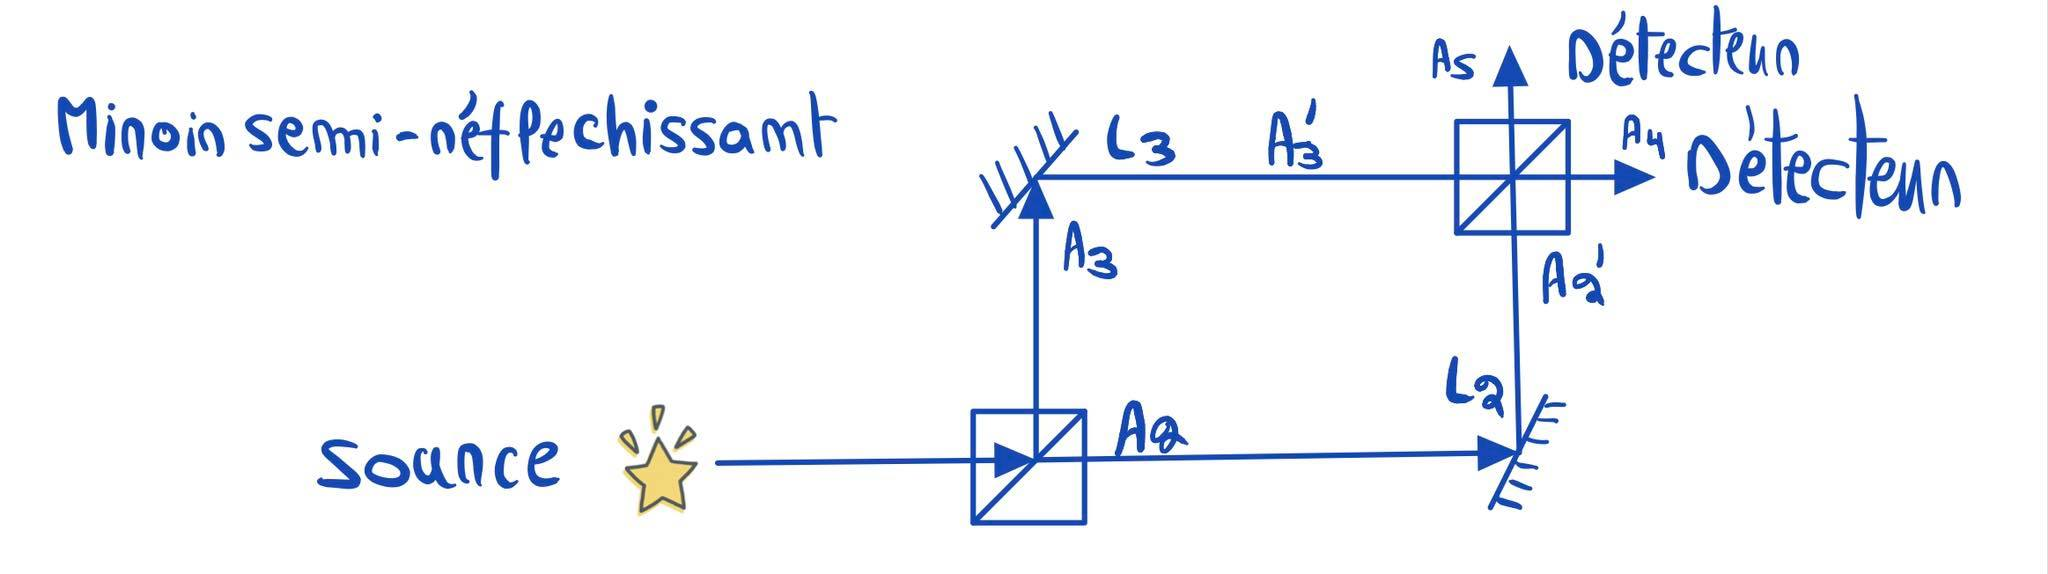
\includegraphics[width=0.80\textwidth]{Mach-Zehnder.png}
    \caption{Représentation du principe de l'interféromètre de Mach-Zehnder. Notons que les longueurs $L_i$ représentent la longueur totale du trajet dans le chemin $i$ suivit.}
    \label{Mach-Zehnder}
    \end{figure}
\end{center}

\subsection{Brève description des détecteurs}
Au niveau des détecteurs, plusieurs chemins sont possibles, comme l'illustre l'image ci-contre.

\begin{center}
    \begin{figure}[h]
    \centering
    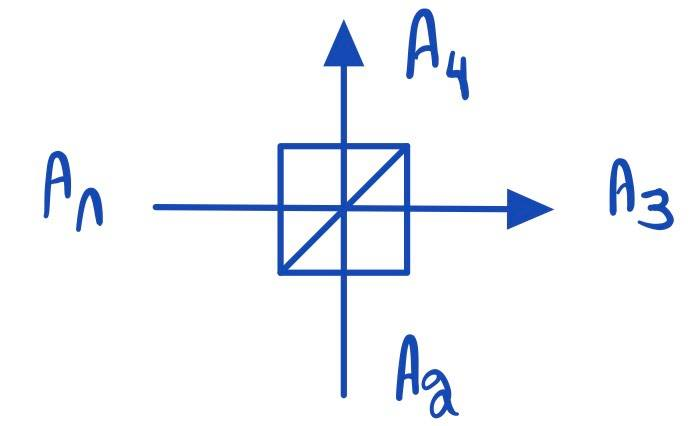
\includegraphics[width=0.50\textwidth]{bean.png}
    \caption{Les ondes incidentes arrivants de $A_1$ et $A_2$ poursuivent leur chemin, respectivement en $A_3$ et $A_4$.}
    \label{Interferometre}
    \end{figure}
\end{center}

Nous avons un miroir semi-transparant. Nous envoyons dessus par le port 1 un faiseau de lumière d'amplitude $A_1$, et d'intensité $I_1 = \norm{A_1}^2$ ; par le port 2, nous envoyons un faisceau d'amplitude $A_2$ et d'intensité $I_2 = \norm{A_2}^2$. \emph{En supposant qu'il n'y a pas de pertes}, nous avons que la somme des intensités entrantes est égale à la somme des intensités sortantes : $I_1 + I_2 = I_3 + I_4$. Puisque les équations de l'électromagnétisme sont linéaires, nous avons $A_3 = \alpha A_1 + \beta A_2$, pour tout $\alpha,\beta\in\mathbb{C}$. Nous pouvons facilement mesurer les valeurs absolues de ces coefficients. En posant $A_2 = 0$, nous pouvons mesurer $I_3$ ; nous trouverons $\norm{\alpha}^2$.

Partons de la description d'une onde plane. Nous aurons
\begin{subequations}
    \begin{equation}
        A_1 (t) = A_1e^{-i\omega t},
    \end{equation}
    \begin{equation}
        A_2 (t) = A_2e^{-i\omega t},
    \end{equation}
\end{subequations}

pour les ondes incidentes, ainsi que
\begin{subequations}
    \begin{equation}
        A_3 (t) = cA_1e^{-i\omega t} + i s A_2e^{-i\omega t}
    \end{equation}
    \begin{equation}
        A_4 (t) = c A_2e^{-i\omega t} + i sA_1e^{-i\omega t}
    \end{equation}
\end{subequations}

pour les ondes sortantes. La discussion précédente nous permet de choisir un des coefficients - soit $\norm{c}^2$ - en choissisant le miroir semi-transparent. Le coefficient $\norm{s}^2$ est alors fixé par

\begin{equation}
\norm{c}^2 + \norm{s}^2 = 1.
\end{equation}

Il nous reste une liberté de phase : nous pouvons redéfinir la phase de $A_1 = e^{i \Phi}A'_1$, et de même pour $A_2, A_3$ et $A_4$. Il s'agit d'une question de convention.

\begin{remark} 
    Par convention, les ondes transmises ne subissent aucun déphasage, là où les ondes réfléchies bénéficient d'un déphasage de $\frac{\pi}{2}$. D'autres conventions sont possibles.
\end{remark}

\begin{remark} 
    Nous pouvons prendre $c = \cos\theta$ et $s = \sin\theta$ pour un argument $\theta$, ce qui explique la notation utilisée. 
\end{remark}

\subsection{Lumière classique}
Pour simplifier, prenons $c = \frac{1}{\sqrt{2}} = s$. Notons que nous pouvons introduire un facteur $e^{ikL}$ tenant compte de la distance parcourue, i.e. un point en $x = 0$ peut-être décrit par $A(t) = Ae^{-i\omega t}$ et un point en $x = L$ peut-être décrit par $A'(t) = Ae^{-i\omega t}e^{ikL}$. Notre détecteur repère le courant électrique $I(t)$ selon $I(t) = e\norm{A(t)}^2$ - soit 

\begin{align*}
A(t) &= Ae^{-i\omega t}	&I_{0} = \norm{A(t_0 = 0)}^2 = \norm{A}^2.
\end{align*}

Nous avons alors que

\begin{align*}
A_2 (t) &= \frac{A(t)}{\sqrt{2}}	&A_3 (t) = i\frac{A(t)}{\sqrt{2}}
\end{align*}

En particulier, nous pouvons écrire les chemins $A_2'$ et $A_3'$ selon:
\begin{subequations}
    \begin{align}
        A'_2 (t) &= A_2 (t)e^{ikL_2}	&A'_3 (t) = A_3 (t)e^{ikL_3}
    \end{align}
\text{De même, les chemins $A_4$ et $A_5$ s'écrivent:}
    \begin{align}
        A_4 &= \frac{1}{\sqrt{2}} (A'_3 + iA'_2) = i\frac{A(t)}{2} (e^{ikL_3} + e^{ikL_2})		&A_5 = \frac{A(t)}{2} (e^{ikL_2} - e^{ikL_3})  
    \end{align}
\end{subequations}

En introduisant le terme $\Delta \Phi = kL_3 - kL_2$, nous pouvons conclure que:
\begin{subequations}
    \begin{align}
        I_4 &= \frac{\norm{A}^2}{4} \norm{e^{ikL_2} + e^{ikL_3}}^2 = \norm{A}^2 \cos^2 \frac{k(L_3-L_2}{2} = \norm{A}^2 \cos^2 \frac{\Delta\Phi}{2}\\
        I_5 &= \norm{A}^2 \sin^2 \frac{\Delta \Phi}{2}
    \end{align}
\end{subequations}

Remarquons que $I_4+I_5 \doteq I_{0}$ - soit $I_0 = \norm{A}^2$, comme prévu. Hourra.

\subsection{Lumière quantique}

Le photon peut suivre plusieurs chemin simultanément : par superposition, nous écrivons l'état comme

\begin{equation}
    \ket{\psi} = \alpha\ket{1}+\beta\ket{2}+\gamma\ket{3}
\end{equation}
Où $\ket{i}$ décrit le photon dans le chemin $i$.\\

Dans un beam splitter tel que décrit par \eqref{Interferometre}, nous décrivons alors les transitions
\begin{align}
    \ket{1} &\rightarrow c\ket{3} + is\ket{4},\\
    \ket{2} &\rightarrow is\ket{3} + c\ket{4}.
\end{align}
Cette transition est décrite par la matrice  $\begin{pmatrix}
c & is\\
is & c
\end{pmatrix}$, unitaire.\\

Soit une mesure dans la base $\ket{1},\ket{2}$ ; donnée par l'était $\ket{\psi} = \alpha\ket{1}+\beta\ket{2}$. Dès lors, les probabilités de détection seront données par $P_1 = \norm{\alpha}^2$ et $P_2 = \norm{\beta}^2$.\\

Il s'ensuit que la decription de l'interféromètre \ref{Interferometre} sera la suivante:

\begin{itemize}
    \item \textbf{Chemins 2 et 3.}
        \begin{equation}
            \ket{\psi} = \frac{1}{\sqrt{2}}\ket{2} + \frac{1}{\sqrt{2}}\ket{3}
        \end{equation}
    \item \textbf{Chemins 2' et 3'.}
        \begin{align}
            \ket{\psi} &= \frac{e^{ikL_2}}{\sqrt{2}}\ket{2'} + \frac{i}{\sqrt{2}}e^{ikL_3}\ket{3'}\\
        \end{align}
    \item \textbf{Chemins 4 et 5.}
        \begin{align}
            \ket{\psi} &= \frac{1}{2} (e^{ikL_2} - e^{ikL_3})\ket{5} + \frac{i}{2}(e^{ikL_2} + e^{ikL_3})\ket{4}
        \end{align}
\end{itemize}

Dès lors,nous avons que les probabilités de détections en 4 et en 5 seront:
\begin{align}
    P_4 &= \cos^2 \frac{\Delta \Phi}{2}\\
    P_5 &= \sin^2 \frac{\Delta \Phi}{2}
\end{align}
\emph{Le photon est simultanément dans les chemins 2 et 3.}\\

Remarquons que si nous supprimons le beam splitter à la fin, les probabilités de présence se réduisent à
\begin{equation}
    P_4 = \frac{1}{2} = P_5
\end{equation}

Les \emph{delayed choice experiment} (Wheeler, 1978) - qui consistent à enlever/remettre le beam splitter, ou à changer la phase $\Delta\Phi$ après que le photon soit entré dans l'interféromètre - nous apprennent que \textbf{toute interprétation ou l'on suppose que le photon "sait à l'avance ce qu'il doit faire", ne tient pas.}

\section{Oscillations de neutrinos}
Une particule est dite élémentaire lorsque sa composition nous est inconnue. L'étude du comportement de ce type de particules fait l'objet de la physique des particules. Le plus récent modèle mathématique décrivant cette réalité est un résultat connu sous le nom de \textit{modèle standard des particules élémentaires}. Un exemple de telle particule est l'électron, rencontré dans les atomes. Il se trouve que le neutrino en est un autre exemple. Notons que la découverte de cette particule est extrêmement récente à l'échelle de l'histoire de la science et de l'humanité : elle a été prédite par Pauli en 1930, et ne fût observée pour la première fois qu'en 1956.\\

Une des propriétés fondamentales du neutrino est qu'elle n'intéragit que très faiblement avec la matière. Aussi, ceci explique pourquoi sa découverte n'est que très récente: il aurait auparavent été tout bonnement impossible de l'observer, en raison de limitation technologiques. Les neutrinos sont produites lors de certaines réactions stellaire; notons de plus qu'il existe 3 "saveurs"\footnote{\color{red}On peut peut-être donner une définition de saveur? Si oui, quoi mettre?} de neutrinos:
\begin{itemize}
    \item Neutrino électronique, noté $\nu_e$ et l'anti-particule associée;
    \item Neutrino muonique, noté $\nu_\mu$ et l'anti-particule associée;
    \item Neutrino tau, noté $\nu_\tau$ et l'anti-particule associée.
\end{itemize}
La plupart des neutrinos observés sur Terre sont produite par le Soleil, selon la réaction
\begin{equation}\label{eq:reaction neutrino}
    p^+ + p^+ \longrightarrow D^+ + e^+ + \nu_e
\end{equation}
où $p^+$ représente un proton, $D^+$ représente \color{red}\textbf{(que représente-t-il?)} \color{black} et où $\nu_e$ et $\bar{\nu}_e$ représentent respectivement le neutrino et l'anti-neutrino électronique. Dans cette réaction, on définit le \textit{nombre leptonique} par la relation
\begin{equation}
    Le = \#e^- + \#\nu_e - (\#e^++\#\bar{\nu}_e)
\end{equation}
\begin{Property}
    Lors d'une intéraction, le nombre leptonique Le constitue une quantité conservée.
\end{Property}

\color{red} Est-il vraiment pertinent d'introduire ce nombre ici, alors qu'il n'est pas utilisé dans la suite de l'application? \color{black}\\

Une fois produite, les neutrinos se propagent presque sans absoption jusqu'à la terre - nous pouvons à présent les mesurer, mais cela reste un exercice non trivial (\textit{et n'est donc pas laissé en exercice pour le lecteur}). \textbf{Nous détectons approximativement la moitié du flux attendu}. \color{red} D'où sort cette information? \color{black} Dans la résolution qui va suivre, nous supposerons que les neutrinos ont une masse (aussi faible soit-elle), et que les états propre de masse ne sont pas les états produits/absorbés lors de son intéraction avec la matière.

\paragraph{Résolution pour une seule espèce de neutrinos}

Supposons que nous ne travaillons qu'avec un neutrino $\nu$ dont nous ne préciserons pas la saveur. Soit $E$ son énergie, et $\Psi(x,t)$ sa fonction d'onde : nous pouvons choisir une onde plane pour la décrire, selon
\begin{equation}
    \Psi(x,t) = e^{-\left(Et-px\right)}
\end{equation}
où nous sommes passés dans le système naturelle d'unité avec $\h = 1 = c$. Dans la limite ultra-relativiste, $E,p >> m$ où l'énergie est donnée par la relation de dispersion
\begin{equation}
    E^2 = m^2 + p^2 \Rightarrow p \approx E-\frac{m^2}{2E}
\end{equation}
Nous pouvons alors réécrire la fonction d'onde sous la forme
\begin{equation*}
    \psi(x,t) = e^{-i\left(E\left[t-x\right]+\frac{m^2}{2E}x\right)} = e^{-iE\left(t-x\right)e^{-i\frac{m^2x}{2E}}}
\end{equation*}
Finalement, cette égalité peut-être écrite sous forme vectorielle:
\begin{equation}\label{eq:fonction d'onde}
    \ket{\psi(x,t)} = e^{-iE\left(t-x\right)e^{-i\frac{m^2x}{2E}}}\ket{\nu}
\end{equation}
où $\ket{\nu}$ dénote l'espèce de neutrino en question.
\paragraph{Résolution pour 2 espèces de neutrinos}
Nous supposons à présent l'existence de deux espèces de neutrino: le neutrino électronique et le neutrino muonique, dénotés $\ket{\nu_e}$ et $\ket{\nu_\mu}$ dans nos conventions. Le soleil produit $\ket{\nu_e}$, et nous ne sommes capable de détecter (sur Terre) que cette dernière.\\

Si nous mesurions un neutrino à un moment quelconque de la propagation, elle aurait une certaine probabilité d'être électronique, et une certaine propabilité d'être muonique. Nous pouvons traduire cela en le fait qu'elle ait une certaine probabilité d'être de masse $m_1$, et une certaine probabilité d'être de masse $m_2$. Nous noterons ces deux états $\ket{\nu_1}$ et $\ket{\nu_2}$.\\

Nous travaillons dans les bases $\left\{\ket{\nu_e},\ket{\nu_\mu}\right\}$ et $\left\{\ket{\nu_1},\ket{\nu_2}\right\}$. Nous sommes donc dans un système à deux niveau, c'est à dire tel que $\dim\mathcal{H} = 2$. Dans ce cas,
\begin{equation}
    \begin{cases}
        \ket{\nu_e} = \cos\theta\ket{\nu_1}+\sin\theta\ket{\nu_2}\\
        \ket{\nu_\mu} = -\sin\theta\ket{\nu_1}+\cos\theta\ket{\nu_2}
    \end{cases}
    \Leftrightarrow
    \begin{cases}
        \ket{\nu_1} = \cos\theta\ket{\nu_e}-\sin\theta\ket{\nu_\mu}\\
        \ket{\nu_2} = \sin\theta\ket{\nu_e}+\cos\theta\ket{\nu_\mu}
    \end{cases}
\end{equation}

\begin{enumerate}
    \item Au temps $t_0 = 0$, le soleil produit un neutrino électronique $\ket{\nu_e}$. On peut exprimer ceci dans la base $\left\{\ket{\nu_e},\ket{\nu_\mu}\right\}$, soit
    \begin{equation*}
        \ket{\psi(t_0,x=0)} = \ket{\nu_e} = \cos\theta\ket{\nu_1}+\sin\theta\ket{\nu_2}.
    \end{equation*}
    \item Le neutrino se propage vers la Terre. Nous exprimons alors ce déplacement dans la base $\left\{\ket{\nu_1},\ket{\nu_2}\right\}$, afin de prévoir les cas de changement spontané de saveur du neutrino. La fonction d'onde peut alors se réécrire sous la forme suivante, en vertue de \eqref{eq:fonction d'onde}.
    \begin{equation*}
        \ket{\psi(t,x)} = e^{-iE\left(t-x\right)}\left[e^{-i\frac{m_1^2}{2E}x}\cos\theta\ket{\nu_1}+e^{-i\frac{m_2^2}{2E}x}\sin\theta\ket{\nu_2}\right]
    \end{equation*}
    \item Finalement, en $x=L$, le neutrino arrive sur Terre. Retournons dans la base des saveurs, afin de pouvoir les discerner. 
    \begin{align*}
        \ket{\psi(t,x=L)} &= e^{-iE\left(t-L\right)}\left[e^{-i\frac{m_1^2}{2E}L}\cos\theta\left\{\cos\theta\ket{\nu_e}-\sin\theta\ket{\nu_\mu}\right\}+e^{-i\frac{m_2^2}{2E}L}\sin\theta\left\{\sin\theta\ket{\nu_e}+\cos\theta\ket{\nu_\mu}\right\}\right]\\
        &= e^{-iE\left(t-L\right)}\left[\left(\cos^2\theta e^{-i\frac{m_1^2}{2E}L}+\sin^2\theta e^{-i\frac{m_2^2}{2E}L}\right)\ket{\nu_e}+\left(e^{-i\frac{m_2^2}{2E}L}-e^{-i\frac{m_1^2}{2E}L}\right)\cos\theta\sin\theta\ket{\nu_\mu}\right]
    \end{align*}
Expérimentalement, nous ne pouvons détecter que les neutrino électronique. Pourtant, la probabilité que le neutron électronique du départ devienne un neutrino muonique est non-nulle, et est donnée par
\begin{align}
    P(NO \; \nu) &= \norm{\braket{\nu_\mu|\psi(t,L)}}^2 = \norm{\left(e^{-i\frac{m_2^2}{2E}L}-e^{-i\frac{m_1^2}{2E}L}\right)\cos\theta\sin\theta}^2 = \sin^22\theta\sin^2\left(\frac{\Delta m^2L}{4E}\right)
\end{align}
où nous avons posé $\Delta m^2 = m_1^2-m_2^2$. Il existe donc une probabilité non-nulle que nous ne puissions pas faire de mesure.
\end{enumerate}

Empiquement, il se trouve que $\sin^22\theta \approx 0.85$ et $\Delta m^2 \approx 8 10^{-5} eV^2$.


% \section{MASER $NH_3$}
% Dans cette section, nous allons discuter d'un appareil fort pratique: le MASER\footnote{Acronyme anglais pour 'Microwave Amplicifaction by Stimulated Emission of Radiation'.} d'ammonium $NH_3$ ; l'un des ancêtres des LASER\footnote{Acronyme anglais pour 'Light Amplification by Stimulated Emission of Radiation'.}

\section{Résonance quantique}

\subsection{Exemple 1 : l'atome de $NH_3$}

\color{red} \textbf{Insérer graphique.} \color{black}

Dans la base $\{\ket{1},\ket{2}\}$, l'Hamiltonien de ce système s'exprime par
\begin{equation}
    H = 
    \begin{pmatrix}
        E_0 & -A\\
        -A & E_0
    \end{pmatrix}
\end{equation}
Il se trouve que dans la base $D = \{\ket{E_0-A},\ket{E_0+A}\}$ des états propres d'énergie, cette matrice est diagonale. Nous observons alors que l'énergie fondamentale $E_0 > E_0-A$. Nous en concluons que si l'atome peut effectivement être stable dans l'état non-dégénéré d'énergie $E_0$, il l'est encore plus dans l'état doublement dégénéré d'énergie $E_0-A$. D'autres exemples similaire existent, tel que celui de la molécule de Benzène.

% \subsection{Ion moléculaire $H_2^+$}

% Bla,bla, ... compléter !

\section{Spin $\frac{1}{2}$}
Ce chapitre consistue une brève introduction à la quantification du moment angulaire. Débutons par une introduction au concept de groupes de rotations.

\subsection{Groupe de rotations}

Considérons l'ensemble des matrices $R \in \mathbb{R}^{3\times 3}$ telle que $R^TR = \mathbb{I}$. Si $\bm{n}$ est un vecteur unitaire de $\mathbb{R}^3$ et $\theta$ un angle, alors $R(\theta,\bm{n}$) est la rotation (dans le sens trigonométrique) autour de l'axe $\bm{n}$ d'angle $\theta$.

\begin{align*}
    R(\theta,x) &= \begin{pmatrix}
    1 & 0 & 0\\
    0 & \cos\theta & -\sin\theta\\
    0 & \sin\theta & \cos\theta
    \end{pmatrix} = \exp (i\theta L_x)			&\text{où } L_x &= \begin{pmatrix}
    0 & 0 & 0\\
    0 & 0 & i\\
    0 & -i & 0
    \end{pmatrix}\\
    R(\theta,y) &= \begin{pmatrix}
    \cos\theta & 0 & \sin\theta\\
    0 & 1 & 0\\
    -\sin\theta & 0 & \cos\theta\\
    \end{pmatrix} = \exp(i\theta L_y)		&\text{où } L_y &= \begin{pmatrix}
    0 & 0 & -i\\
    0 & 0 & 0\\
    i & 0 & 0
    \end{pmatrix}\\
    R(\theta,z) &= \begin{pmatrix}
    \cos\theta & -\sin\theta & 0\\
    \sin\theta & \cos\theta & 0\\
    0 & 0 & 1
    \end{pmatrix} = \exp(i\theta L_z)		&\text{où } L_z &= \begin{pmatrix}
    0 & i & 0\\
    -i & 0 & 0\\
    0 & 0 & 0
    \end{pmatrix}
\end{align*}
Nous avons alors que $R(\theta,\bm{n}) = \exp (i\theta\bm{n}\cdot\bm{L})$, où $\bm{n}\cdot\bm{L} = n_iL_i$. Les vecteurs $L_x,L_y,L_z$ sont les \emph{générateurs du $\mathcal{G}$roupe des $\mathcal{R}$otations}.

\begin{Property}
    Les générateurs du groupe des rotations commutent selon
    \begin{equation}
        [L_i,L_j] = L_k
    \end{equation}
    pour tout $i,j \neq k$. 
\end{Property}

En physique, de nombreux objets (et non pas seulement les vecteurs) sont invariants ou se transforment sous l'effet d'une rotation. Une autre représentation du $\mathcal{G}$roupe des $\mathcal{R}$otations est l'ensemble des 3 opérateurs $J_x,J_y,J_z$ tels que $[J_x,J_y] = J_z$ (et toutes ses permutations cycliques) et tel que, sous toute rotation d'angle $\theta$ autour de $\bm{n}$, un état $\ket{\psi}$ se transforme en
\begin{equation}
\ket{\psi} \rightarrow \exp(i\theta\bm{n}\cdot\bm{J})\ket{\psi}
\end{equation}

\begin{exemple}Les opérateurs
\begin{itemize}
\item $J_x = yp_z - zp_y$
\item $J_y = zp_x - xp_z$
\item $J_z = xp_y - yp_x$
\end{itemize}
sont des exemples de représentation du $\mathcal{G}$roupe des $\mathcal{R}$otations.
\end{exemple}
Un système est invariant par rotation si
\begin{align}
\exp (-itH) \exp (i\theta \bm{n}\cdot\bm{J})\ket{\psi} &= \exp (i\theta \bm{n}\cdot\bm{J})\exp (-itH) \ket{\psi}			&\forall \ket{\psi},\forall \bm{n},\theta,t
\end{align}
Cela revient à dire que \emph{faire une rotation} et ensuite \emph{évoluer dans le temps} est identique à \emph{évoluer dans le temps} et puis \emph{faire une rotation}.

\begin{Property} 
    Pour tout petit angle sur des temps négigeables,  
    \begin{equation}
        [H,J_x] = [H,J_y] = [H,J_z] = 0.
    \end{equation}
\end{Property}
Les conséquences en sont nombreuses. Voici quelques exemples.
\begin{Property}
    Si $\ket{\psi(t)}$ est une solution de l'équation de Schrödinger \eqref{Schrodinger}, alors 
    \begin{equation}
        \frac{d}{dt}\braket{\psi(t)|J_i|\psi(t)} = 0
    \end{equation}
    Nous avons en particulier que $\braket{\psi(t)|J_i|\psi(t)} = \braket{\psi(0)|J_i|\psi(0)}$.
\end{Property}

\begin{Property}
    Si $\ket{\psi_0}$ est un vecteur propre de $J_i$ tel que $J_i\ket{\psi_0} = j\ket{\psi_0}$, alors le vecteur $\ket{\psi(t)} = e^{-iHt}\ket{\psi_0}$ est également un vecteur propre de $J_i$:
    \begin{equation}
        J_i\ket{\psi(t)} = j\ket{\psi(t)}.
    \end{equation}
\end{Property}
Le théorème d'Emmy Nöther permet de montrer que la symmétrie de rotation implique la conservation d'une quantité : le moment angulaire.


\subsection{Quantification du moment angulaire}
\begin{theorem}
Soit $[J_x,J_y] = iJ_z$. Nous avons alors que les valeurs propres de $J_z$ est un demi-entier: $0,\frac{1}{2}, 1, \frac{3}{2}, ...$.
\begin{equation*}
J_z \ket{\psi} = m\ket{\psi}
\end{equation*}
\end{theorem}

\begin{theorem}
Il existe une représentation non triviale du $\mathcal{G}$roupe des $\mathcal{R}$otations par des matrices $d\times d$. Dans ce cas, $J_z = -\frac{d}{2}, -\frac{d}{2}+1,...,+\frac{d}{2}$.
\end{theorem}
\begin{exemple}
Le cas le plus simple est celle des matrices de Pauli (matrices $2\times 2$):
\begin{center}
\begin{tabular}{c|c|c}
$\sigma_x = \begin{pmatrix}
0 & 1\\
1 & 0
\end{pmatrix}$ & $\sigma_x = \begin{pmatrix}
0 & -i\\
i & 0
\end{pmatrix}$ & $\sigma_x = \begin{pmatrix}
1 & 0\\
0 & -1
\end{pmatrix}$\\
$J_x = \frac{1}{2}\sigma_x$ & $J_y = \frac{1}{2}\sigma_y$ & $J_z = \frac{1}{2}\sigma_z$
\end{tabular}
\end{center}
Nous pouvons vérifier que les différentes relations démontrées ci-dessus sont respectées (exercice).
\end{exemple}

En particulier, nous pouvons vérifier que 
\begin{center}
    \begin{tabular}{c|c|c|c}
        $\{\sigma_a,\sigma_b\} = 2i\varepsilon_{abc}\sigma_c$ & $\{\sigma_a,\sigma_b\} = 2\sigma_{ab}\hat{I}$ & $Tr(\sigma_a) = 0$ & $\sigma_a\sigma_b = \delta_{ab}\hat{I}+i\varepsilon_{abc}\sigma_c$
    \end{tabular}
\end{center}

Les matrices de Pauli sont de valeur propres $\pm 1$. Les vecteurs propres associés sont
\begin{center}
    \begin{tabular}{c|c}
        $\psi_x^+ = \frac{1}{\sqrt{2}} \begin{pmatrix}
            1\\
            1
        \end{pmatrix}$ & $\psi_x^- = \frac{1}{\sqrt{2}} \begin{pmatrix}
            -1\\
            1
        \end{pmatrix}$\\
        $\psi_y^+ = \frac{1}{\sqrt{2}} \begin{pmatrix}
            -1\\
            1
        \end{pmatrix}$ & $\psi_y^- = \begin{pmatrix}
            i\\
            i
        \end{pmatrix}$\\
        $\psi_z^+ = \begin{pmatrix}
            1\\
            0
        \end{pmatrix} = \ket{\uparrow}$ & $\psi_z^- = \begin{pmatrix}
            0\\
            1
        \end{pmatrix} = \ket{\downarrow}$
    \end{tabular}
\end{center}

Introduisons le vecteur unitaire associé aux coordonnées sphériques $\bm{n} = \left(\sin\theta\cos\varphi,\sin\theta\sin\varphi,\cos\theta\right)$. Observons que 
\begin{equation}
    \bm{n}\cdot\bm{\sigma} = \begin{pmatrix}
        \cos\theta & \sin\theta e^{-i\varphi}\\
        \sin\theta e^{i\varphi} & -\cos\theta
    \end{pmatrix}
\end{equation}
De même, observons que $\begin{pmatrix}
    \cos\frac{\theta}{2}\\
    \sigma\frac{\theta}{2}e^{i\varphi}
\end{pmatrix}$ est le vecteur propre de valeur propre $+1$. Nous pouvons réécrire, dans la base des vecteurs up and down,
\begin{equation}
    \begin{pmatrix}
        \cos\frac{\theta}{2}\\
        \sigma\frac{\theta}{2}e^{i\varphi}
    \end{pmatrix} = \cos\frac{\theta}{2}\ket{\uparrow}+\sin\frac{\theta}{2}e^{i\varphi}\ket{\downarrow}
\end{equation}

Les particules élémentaires ont un spin $1/2$. Elles sont munies d'un espace de Hilbert de dimension 2, se transformant sous rotations par $e^{i\frac{\theta}{2}\bm{n}\cdot\bm{\sigma}}$.

\end{document}